\documentclass[a4paper,12pt]{article}
\usepackage{mathtools}
\usepackage{graphicx,url}
\usepackage[english]{babel}

\graphicspath{{.}{images/}}
\pdfimageresolution=600

\begin{document}

\title{QMClique: A Proposal and Questions for Quantum Maximal Clique Algorithm}
\author{Gustavo C. G. van Erven\footnote{gustavo.erven@cgu.gov.br}}
\maketitle

\begin{abstract}
	Finding cliques in graphs is a well known computing problem. These notes present an algorithm for maximal cliques and a research question for its implementation in a quantum computer. 
\end{abstract}

\section{Definitions}

A Graph $G(V,E)$ is a set of vertices $V = \{v_1,v_2,\dots,v_n\}$ with a set $E$ of relations between them, $E = \{e_1,e_2,\dots,e_m\}$ and $e_i = (u,v) | u,v \in V$.

A Clique is a subgraph of $G(V,E)$, in which all vertices are connected to one another.

Theorem: Let $W_i$ be the set of all adjacent vertices for vertex $i$, plus the union with $\{v_i\}$, $W_i = V_{adj(i)} \cup \{v_i\}$, if C is a maximal clique of size k:
\begin{equation}\label{eq:clique}
C = \{\{v_i\} \cup \{v_{i+1}\} \cup \dots \cup \{v_k\}\} = \{W_i \cap W_{i+1} \cap \dots \cap W_{k}\}
\end{equation}

The right side of Equation~\ref{eq:clique} has all vertices in the clique $C$. Therefore, they must be presented in the left side, because all vertices in a clique are connected to each other. The intersection has only vertices that are in the clique, because they are the elements in common between all of them. If any vertex is on the left side and not on the union, the vertex will be a common vertex, and the right side will not be complete. 

If there is a vertex in the union that is not in the maximal clique, it will not be presented in the intersection, because it will not be connected to all elements of the set.

\section{Checking a maximal clique}

Let $H_i$ be the set $V_{adj(i)} \cup \{v_i\}$, we can represent it as a vector, such as the one shown in Equation~\ref{eq:vech}, where $e_i$ is equal to 1 if the vertex $i$ is connected to the node in the index position.

\begin{equation}\label{eq:vech}
W_i = 
	\begin{bmatrix}
		e_{1} \\
		e_{2} \\
		\vdots  \\
		e_{n}
	\end{bmatrix}
\end{equation}

Therefore, the set with all vectors $H_i$ is equivalent to the adjacent matrix below.

\begin{equation}
W = 
	\begin{bmatrix}
	1 & e_{1,2} & \cdots & e_{1,n} \\
	e_{2,1} & 1 & \cdots & e_{2,n} \\
	\vdots  & \vdots  & \ddots & \vdots  \\
	e_{n,1} & e_{n,2} & \cdots & 1 
	\end{bmatrix}
\end{equation}

Let $A$ be a vector that represents the presence of the vertex $v_i$ when $a_i$ is set to 1 or otherwise to 0, such that:

\begin{equation}
A = 
\begin{bmatrix}
a_{1} \\
a_{2} \\
\vdots  \\
a_{n}
\end{bmatrix}
\end{equation}

And $A_i$ a vector composed by $n$ elements, of $a_i$, such that $a_i \in A$:

\begin{equation}
A_i = 
\begin{bmatrix}
a_{i} \\
a_{i} \\
\vdots  \\
a_{i}
\end{bmatrix}
\end{equation}

According to Equation~\ref{eq:clique}, if a vector $A$ is given, we can check if it is a maximal clique by verifying if the intersection of vectors $W_i$ is equal to $A$. The intersection can be calculated with AND ports.

\begin{equation}
	\text{A is a maximal clique iff is equal to } W_i \land W_{i+1} \land \dots \land W_k
\end{equation}

Now, we can compute a true value which represents if the input vector $A$ is a maximal clique. At first, if $a_i$ is present, the vector $W_i$ must be used. Otherwise, the presence of the vertex must be ignored. We can ignore the vector by changing all the values to 1, then it will not influence the AND operations. The Equation~\ref{ex:removea1} presents an example for a $W_i$ vector. 

\begin{align}
	\neg A_i \lor (A_i \land W_i) \\
	(\neg A_i \lor A_i) \land (\neg A_i \lor W_i) \\
	\neg A_i \lor W_i \label{ex:removea1}
\end{align}

Therefore, if $a_1$ is 0, all the values in $W_i$ will be changed to 1, and it will not affect the AND operations. Now we can generalize to check an input $A$ over all vectors in $W$. Let $O$ be the output vector for the AND operations, thus:

\begin{equation}
	O = (\neg A_1 \lor W_1) \land (\neg A_2 \lor W_2) \land \dots \land (\neg A_n \lor W_n)
\end{equation}

Therefore, $O_i$ is the result for the element $a_i$, where $w_{ij}$ is the element $j$ for the vector $W_i$:

\begin{equation}
O_i = (\neg a_1 \lor w_{11} \land (\neg a_2 \lor w_{21}) \land \dots \land (\neg a_n \lor w_{n1})
\end{equation}

Now, $A$ will be a clique if the output $O$ is equal to $A$. We can summarize it through a single value. Let $R$ be a boolean variable, such that:

\begin{align}
	U = (O \oplus \neg A)\\
	R = u_1 \land u_2 \land \dots \land u_n\\
	R = (o_1 \oplus \neg a_1) \land (o_2 \oplus \neg a_2) \land \dots \land (o_n \oplus \neg a_n)
\end{align}

Therefore, if $R$ is true, the vector input $A$ is a maximal Clique. Note that, if $A$ is a subset of maximal Clique, $R$ will be false because all vertices with $a_i = 0$ will have their values changed to 1. Therefore, if a node $i$ is not present, but it is adjacent to the selected vertices in $A$, the output value will be true for $O_i$, and the final verification will return false, considering that $O_i = 1$ and $a_i = 0$.

If the algorithm is implemented in a program, the time complexity will be $O(n^2)$, since we need $n$ operation for each $n$ vertex to generate the $O$ vector, and more $n$ operations to calculate $R$.

The code was verified in a R script and can be found online\footnote{https://github.com/gvanerven/quantum/tree/master/testOpClique}.
\section{Using Quantum ports}

The algorithm can be implemented in a quantum computer through the use of the Toffoli gate. The Equation~\ref{ex:removea1} can be modified to make the implementation easier, as shown in Equation~\ref{ex:remtof}.

\begin{equation}
	\neg A_i \lor W_i = 1 \oplus A_i W_i \label{ex:remtof}
\end{equation}

The AND port can be implemented with a Toffoli gate as presented in Equation~\ref{ex:andtof} 

\begin{equation}
	A \land B = 0 \oplus AB \label{ex:andtof}
\end{equation}

These gates can replace the boolean operations in the maximal clique algorithm. A Hadamard gate can be used in the input vector $A$ to create a superposition with all possible values.

The Figure 1 presents an implementation for a two-vertices graph without edges. The qubits are:

\begin{itemize}
	\item Q1 and Q2: $A$;
	\item Q3 and Q4: $W_1$;
	\item Q5 and Q6: $W_2$;
	\item Q7: $1 \oplus a_1 w_{11}$;
	\item Q8: $1 \oplus a_2 w_{21}$;
	\item Q9: $1 \oplus a_1 w_{12}$;
	\item Q10: $1 \oplus a_2 w_{22}$;
	\item Q11: $o_{1}$;
	\item Q12: $o_{2}$;
	\item Q13: $R$;
	\item Q14: Qubit set to $|1\rangle$. It is used to change the $R$ state to $|1\rangle$ and verify if it forces the collapse of $A$ to a maximal clique state; 
\end{itemize}

\begin{figure}[!ht]
	\label{fig:qcircuit}
	\centering
	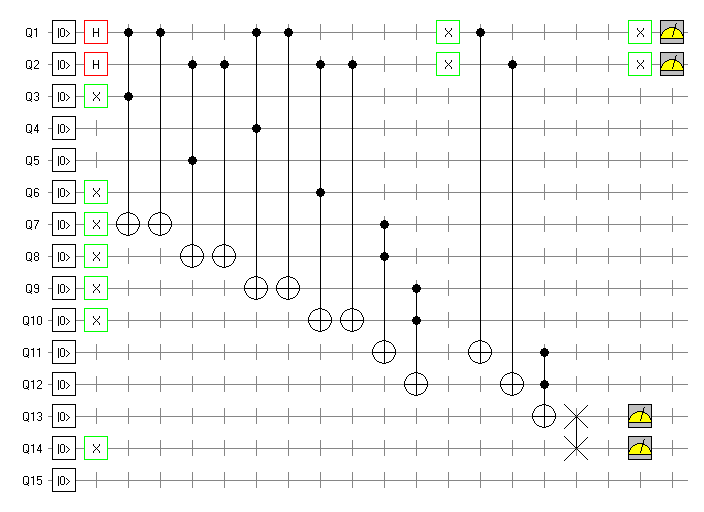
\includegraphics[width=1\textwidth]{qclique}
	\caption{Quantum circuit for a graph with two-vertices.}
\end{figure}

The $W$ matrix for this example is $\bigl(\begin{smallmatrix}
1&0 \\ 0&1 \end{smallmatrix} \bigr)$ and must be true only for $\bigl(\begin{smallmatrix} 1\\0 \end{smallmatrix} \bigr)$ and $\bigl(\begin{smallmatrix} 0\\1 \end{smallmatrix} \bigr)$ inputs.

Note that it will be necessary $n$ qubits for $A$, $n^2$ qubits for $W$, $n^2$ qubits to keep the $(1 \oplus A_i W_i)$ operations, $n$ qubits for the $O$ vectors and one for the result $R$.

A simulation created with libquantum had as output only true states of clique values when it was measured. The circuit used is shown in Figure 2.

\begin{figure}[!ht]
	\label{fig:qcircuitnctr}
	\centering
	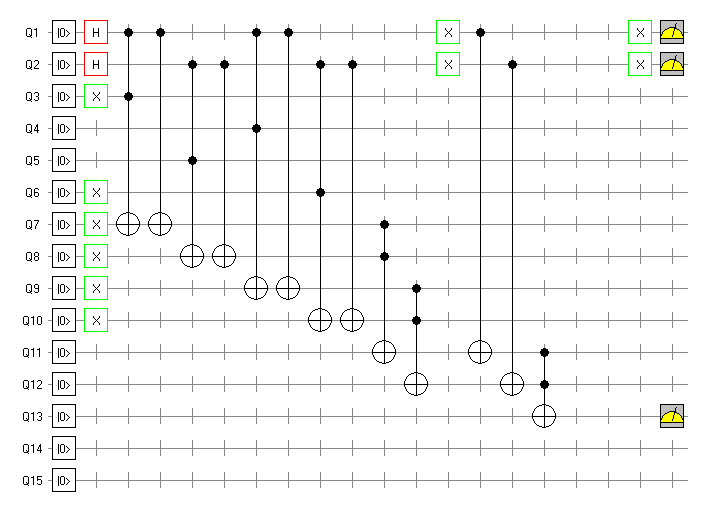
\includegraphics[width=1\textwidth]{qcliquencontr}
	\caption{Quantum circuit for a graph with two-vertices and a measure without a qubit to force output.}
\end{figure}

The simulation was made as well for two qubits and the source code can be found online\footnote{https://github.com/gvanerven/quantum/tree/master/libquantum\_qmclique}

\pagebreak
\section{Conclusions and Question}

The algorithm to verify a maximal clique can be implemented in a quantum computer using Toffoli gates. The Hadamard gate can be used to create a superposition in the input vector $A$. However, we are only interested in values that make $R$ true, which implies in a maximal clique. \textbf{The question is: is there an entangle state that we can use to force the result $R$ to be true and makes $A$ collapse to a maximal clique? Could the swap gate X do this? And if it exists, is there a way to take only the maximum cliques superpositions?}

\end{document}